\documentclass[10pt]{beamer}
\beamertemplatenavigationsymbolsempty
\setbeamertemplate{footline}[page number]{}
\usetheme{Madrid}
\usepackage{appendixnumberbeamer}
\usepackage{amssymb}
\usepackage{amsthm}
\usepackage{bbm}
\usepackage[normalem]{ulem}  % for \sout
\newcommand{\ones}{\mathbf{1}}
\newcommand{\indep}{\rotatebox[origin=c]{90}{$\models$}}
\usepackage{qrcode}

%% === basic packages ===
\usepackage{latexsym,multirow}
\usepackage{amssymb,amsmath,bm}
\usepackage{graphicx}
\usepackage[color,all,import,arrow]{xy}
\usepackage{enumerate}
\usepackage{booktabs}
\usepackage{transparent}
\usepackage{tikz}
\usepackage{graphicx}
\usetikzlibrary{calc}


\theoremstyle{plain}
\newtheorem{assumption}{Assumption}
\newtheorem{property}{Property}
\newtheorem{proposition}{Proposition}
\newtheorem{remark}{Remark}
\newtheorem{defi}{Definition}
\newtheorem{thm}{Theorem}




\usepackage{colortbl}  % Required for \rowcolor
\usepackage{xcolor} 

%% == tikz
\usepackage{tikz}
\usepackage{inputenc}
\usetikzlibrary{shapes,arrows,trees,fit,positioning,shapes.misc,calc}

% === some special symbols
\newcommand{\argmax}{\operatornamewithlimits{argmax}}
\newcommand{\argmin}{\operatornamewithlimits{argmin}}
\newcommand{\ind}{\mbox{$\perp\!\!\!\perp$}}
\newcommand{\nind}{\mbox{$\not\perp\!\!\!\perp$}}


\newcommand{\cX}{\mathcal{X}}

\newcommand{\hbx}{\bar{\bm{x}}}
\newcommand{\hbX}{\overline{\bm{X}}}
\newcommand{\hbz}{\bar{\bm{z}}}
\newcommand{\hbZ}{\overline{\bm{Z}}}

\newcommand{\bx}{\bm{x}}
\newcommand{\bX}{\bm{X}}
\newcommand{\ubX}{\underline{\bm{X}}}
\newcommand{\td}{\text{d}}
\newcommand{\bZ}{\bm{Z}}
\newcommand{\ubZ}{\underline{\bm{Z}}}
\newcommand{\bD}{\bm{D}}
\newcommand{\cD}{\mathcal{D}}
\newcommand{\ubD}{\underline{\bm{D}}}
\newcommand{\ucD}{\underline{\mathcal{D}}}
\newcommand{\bz}{\bm{z}}
\newcommand{\ubz}{\underline{\bm{z}}}
\newcommand{\bd}{\bm{d}}
\newcommand{\ubd}{\underline{\bm{d}}}
\newcommand{\bY}{\bm{Y}}
\newcommand{\ubY}{\underline{\bm{Y}}}
\newcommand{\ucY}{\underline{\mathcal{Y}}}
\newcommand{\by}{\bm{y}}
\newcommand{\uby}{\underline{\bm{y}}}
\newcommand{\cY}{\mathcal{Y}}
\newcommand{\add}{\textsc{Add}}
\newcommand{\std}{\textsc{Std}}
\newcommand{\cof}{\textsc{Cof}}

\newcommand{\oD}{\overline{D}}
\newcommand{\oY}{\overline{Y}}

\newcommand{\bS}{\bar{S}}
\newcommand{\bs}{\bar{s}}
\newcommand{\Ss}{\mathcal{S}}
\newcommand{\N}{\mathbb{N}}
\newcommand{\E}{\mathbb{E}}
\newcommand{\R}{\mathbb{R}}
\newcommand{\bI}{\bm{I}}
\newcommand{\bH}{\bm{H}}
\newcommand{\bM}{\bm{M}}
\newcommand{\bP}{\bm{P}}
\newcommand{\bQ}{\bm{Q}}
\newcommand{\bV}{\bm{V}}
\newcommand{\bU}{\bm{U}}
\newcommand{\bW}{\bm{W}}
\newcommand{\bw}{\bm{w}}
\def\independenT#1#2{\mathrel{\rlap{$#1#2$}\mkern2mu{#1#2}}}
\DeclareMathOperator{\sgn}{sgn}
\DeclareMathOperator{\diag}{diag}
\providecommand{\norm}[1]{\lVert#1\rVert}


\newcommand{\cU}{\mathcal{U}}

\newcommand{\bepsilon}{\bm{\epsilon}}
\newcommand{\boldeta}{\bm{\eta}}
\newcommand{\bC}{\bm{C}}
\newcommand{\bl}{\bm{\ell}}
\newcommand{\ATT}{\mathrm{ATT}}
\newcommand{\Yone}{Y(1)}
\newcommand{\Yzero}{Y(0)}
\newcommand{\ATE}{\mathrm{ATE}}
\usepackage{booktabs,tabularx}
\newcommand{\Var}{\mathrm{Var}}
\newcommand{\Cov}{\mathrm{Cov}}


% BK: Added Userpackages and Commands
\usepackage{dsfont}
\usepackage{caption}
\usepackage{tikz-cd}
\usetikzlibrary{arrows.meta}

\newcommand{\lt}{\left}
\newcommand{\rt}{\right}
\newcommand{\indicator}[1]{\mathds{1}{\left\{ #1 \right\}}}
\newcommand{\prb}[1]{\mathbb{P}{\left( #1 \right)}}
\newcommand{\prbcond}[2]{\mathbb{P}{\left( #1 \mid #2 \right)}}
\newcommand{\Eb}[1]{\mathbb{E}{\left[ #1 \right]}}
\newcommand{\Ebcond}[2]{\mathbb{E}{\left[ #1 \mid #2 \right]}}
\newcommand{\indist}{\overset{d}{\to}}
\newcommand{\inprob}{\overset{p}{\to}}
\newcommand{\as}{\overset{a.s.}{\to}}
\newcommand{\Nb}[1]{\mathcal{N}{\left( #1 \right)}}
\newcommand{\abs}[1]{\left|#1\right|}
\newcommand{\cF}{\mathcal{F}}

\usepackage[style=authoryear]{biblatex}

% Add bib resource
\addbibresource{references.bib}


\usepackage{booktabs}
\usepackage[scale=2]{ccicons}

\usepackage{pgfplots}
\usepgfplotslibrary{dateplot}

\usepackage{xspace}
\newcommand{\themename}{\textbf{\textsc{metropolis}}\xspace}


\title{Final Review Lecture STAT 286}
\author{Benedikt Koch}
\date{Dezember 8th, 2025}
\begin{document}

\begin{frame}[plain]

  \maketitle

\end{frame}


\AtBeginSection[]
{
  \begin{frame}{Outline}
    \tableofcontents[currentsection]
  \end{frame}
}


\section{Observational Studies}

\begin{frame}{Tablets and Test Scores}
  \begin{itemize}
    \item \textbf{Goal}: estimate causal effect of providing tablets on test scores
    \pause
    \item Observational setting: schools decide themselves whether to adopt tablets.
    \pause
    \item Confounding: Wealthier schools are both
    \begin{itemize}
      \item more likely to adopt tablets, and
      \item have higher test scores (tutoring, staffing, etc.).
      \item Confounding in treatment \textbf{and} outcome (one would be ok).
    \end{itemize}
    \pause
    \item We suspect that
    \[
      \mathbb{E}[Y_i \mid T_i=1] - \mathbb{E}[Y_i \mid T_i=0] \neq \mathbb{E}[Y_i(1)-Y_i(0)].
    \]
  \end{itemize}
\end{frame}

\begin{frame}{Assumption I: Super-Population}
  \begin{itemize}
    \item For each unit \(i=1,\dots,n\), we observe 
    \begin{itemize}
        \item covariates \(X_i\),
        \item treatment \(T_i \in \{0, 1\}\),
        \item outcome \(Y_i\).
    \end{itemize}
    \pause
    \item \textbf{Super-population assumption}:
    \[
      \{X_i, T_i, Y_i(0), Y_i(1)\}_{i=1}^n \overset{\text{i.i.d.}}{\sim} \mathbb{P}^*.
    \]
    \pause
    \item In the tablet example:
    \begin{itemize}
      \item \(X_i\): wealth characteristics of school \(i\),
      \item \(T_i\): indicator that school \(i\) adopts tablets,
      \item \(Y_i(t)\): test score that would be observed for school \(i\) if \(T_i=t\).
    \end{itemize}
  \end{itemize}
\end{frame}

\begin{frame}{Assumption II: SUTVA}
  \textbf{Assumption 1 (SUTVA).}
  \begin{itemize}
    \item \emph{No interference:}
    \[
      Y_i(T_1,\dots,T_n) = Y_i(T_i).
    \]
    Tablet adoption of other schools don't affect school $i$. Student's with tablets don't move to schools without.
    \vspace{0.5em}
    \pause
    \item \emph{Consistency:}
    \[
      Y_i = Y_i(T_i).
    \]
    All tablets are treated the same. No adopted tablet is significantly different (more features etc.)
  \end{itemize}
\end{frame}

\begin{frame}{Strong Ignorability / Unconfoundedness}
  \textbf{Assumption 2 (Strong Ignorability / Unconfoundedness).}
  \[
    \{Y_i(1),Y_i(0)\} \indep T_i \mid \bX_i.
  \]
  \pause
  \begin{itemize}
    \item Conditional on pre-treatment covariates \(\bX_i\), treatment is ``as good as randomized.''
    \item Intuition: after conditioning on \(\bX_i\), there are \textbf{no unobserved confounders} that jointly affect \(T_i\) and \(Y_i\).
  \end{itemize}
  \vspace{0.3cm}
  \pause
  \textbf{Tablet example.}
  \begin{itemize}
    \item Suppose \(X_i =\) Wealth 
    \item Within each wealth level, schools with and without tablets differ only by treatment, not by other unobserved factors.
  \end{itemize}
\end{frame}

\begin{frame}{Ignorability DAG}
    \begin{center}
\begin{minipage}{0.47\linewidth}
\centering
\textit{Ignorability holds}
\[
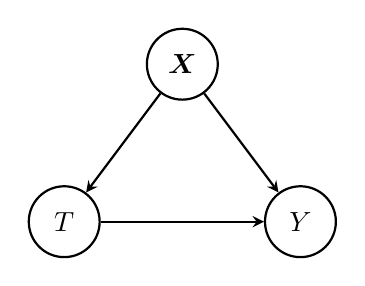
\begin{tikzpicture}[
    >=stealth,
    line width=0.8pt,
    every node/.style={circle, draw, minimum size=9mm, inner sep=0pt}
]
  % nodes
  \node (T) at (1,0)      {$T$};
  \node (Y) at (4,0)    {$Y$};
  \node (X) at (2.5, 2) {$\bX$};

  % edges
  \draw[->] (X) -- (Y);
  \draw[->] (X) -- (T);
  \draw[->] (T) -- (Y);
\end{tikzpicture}
\]
No unmeasured confounding given $\bX$.
\end{minipage}\hfill
\begin{minipage}{0.47\linewidth}
\centering
\textit{Ignorability violated}
\[
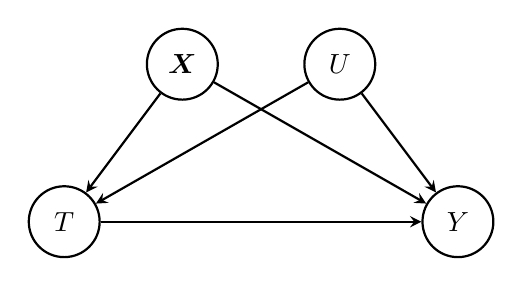
\begin{tikzpicture} [>=stealth,
    line width=0.8pt,
    every node/.style={circle, draw, minimum size=9mm, inner sep=0pt}]
  \node (T) at (1,0)      {$T$};
  \node (Y) at (6,0)    {$Y$};
  \node (X) at (2.5, 2) {$\bX$};
  \node (U) at (4.5, 2) {$U$};
  
  \draw[->] (X) -- (T);
  \draw[->] (X) -- (Y);
  \draw[->] (U) -- (T);
  \draw[->] (U) -- (Y);
  \draw[->] (T) -- (Y);
\end{tikzpicture}
\]
Unmeasured confounding given $\bX$.
\end{minipage}
\end{center}
\begin{itemize}
    \item If \(U\) exists and affects both \(T\) and \(Y\), then \(\{Y(1),Y(0)\} \not\!\indep T \mid \bX\); estimates that omit \(U\) are biased.
    \item Tablet example: $U$ parental involvement
\end{itemize}
\end{frame}

\begin{frame}{Observational / Causal DAG}
    \begin{center}
\begin{minipage}{0.47\linewidth}
\centering
\textit{Observational}
\[
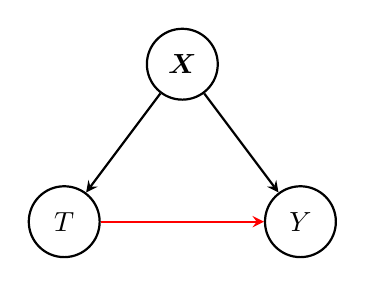
\begin{tikzpicture}[
    >=stealth,
    line width=0.8pt,
    every node/.style={circle, draw, minimum size=9mm, inner sep=0pt}
]
  % nodes
  \node (T) at (1,0)      {$T$};
  \node (Y) at (4,0)    {$Y$};
  \node (X) at (2.5, 2) {$\bX$};

  % edges
  \draw[->] (X) -- (Y);
  \draw[->] (X) -- (T);
  \draw[->, red] (T) -- (Y);
\end{tikzpicture}
\]
$T$ affects $Y$.
\end{minipage}\hfill
\begin{minipage}{0.47\linewidth}
\centering
\textit{Causal}
\[
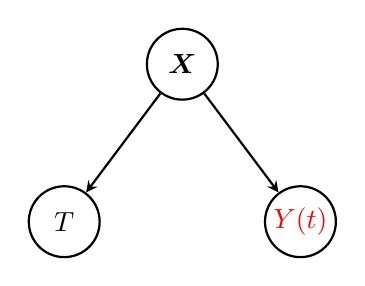
\begin{tikzpicture}[
    >=stealth,
    line width=0.8pt,
    every node/.style={circle, draw, minimum size=9mm, inner sep=0pt}
]
  % nodes
  \node (T) at (1,0)      {$T$};
  \node (Y) at (4,0)    {\textcolor{red}{$Y(t)$}};
  \node (X) at (2.5, 2) {$\bX$};

  % edges
  \draw[->] (X) -- (Y);
  \draw[->] (X) -- (T);
\end{tikzpicture}
\]
$T$ affects $Y(t)$ only through $\bX$.
\end{minipage}
\end{center}
\vspace{0.5em}
\begin{itemize}
    \item By setting $Y$ to level $T = t$ ($Y \to Y(t)$), we remove the arrow from $T$ to $Y$.
    \item All effects of $T$ to $Y$ go through $\bX$.  Conditioning \emph{blocks} that path.
    \item Only condition on confounder, never on collider 
    \item Rule of thumb: Arrow must go into $Y$.
\end{itemize}
\end{frame}


\begin{frame}{Strong Overlap}
  \textbf{Assumption 3 (Strong Overlap).}
  \[
    \exists\,\eta \in \Bigl(0,\tfrac{1}{2}\Bigr) \text{ s.t. } \eta < e(\bx) = \Pr(T=1 \mid \bX = \bx) \le 1-\eta
    \quad\text{for all } \bx.
  \]
  \pause
  \begin{itemize}
    \item Every covariate profile has positive probability of being treated and untreated.
    \item Without overlap, we lack observed counterfactuals:
    \pause
    \begin{itemize}
      \item if \(e(\bx)=1\), we never see controls at \(\bX=\bx\);
      \item if \(e(\bx)=0\), we never see treated units at \(\bX=\bx\).
    \end{itemize}
  \end{itemize}
  \vspace{0.5cm}
  \pause
  \textbf{Tablet example.}
  \begin{itemize}
    \item With \(X=\) Wealth, strong overlap requires that at every wealth level there are both tablet and non-tablet schools.
  \end{itemize}
\end{frame}

\begin{frame}{Ignorability vs.\ Overlap: A Tension}
  \textbf{In observational studies, we rely on both:}
  \begin{itemize}
    \item \textbf{Ignorability:} \(\{Y(1),Y(0)\} \indep T \mid \bX\).
    \item \textbf{Overlap:} \(\eta < \Pr(T=1 \mid \bX) \le 1-\eta\).
  \end{itemize}
  \pause
  \vspace{0.5cm}
  \begin{itemize}
    \item Adding more covariates to \(\bX\)
    \begin{itemize}
      \item makes ignorability more plausible (less risk of omitted confounders),
      \item but makes overlap less plausible: treatment becomes more predictable and \(e(\bX)\) gets closer to 0 or 1.
    \end{itemize}
  \end{itemize}
\end{frame}

\begin{frame}{Identification: ATE}
\small
Under these assumptions we have
\begin{align*}
  \uncover<1->{%
    &\E\bigl[Y_i(1) - Y_i(0)\bigr]
  }\\[0.3em]
  \uncover<2->{%
    &= \E\Bigl[\E\bigl[Y_i(1) - Y_i(0) \mid \bX_i\bigr]\Bigr]
    \qquad \text{(LIE)}
  }\\[0.3em]
  \uncover<3->{%
    &= \E\Bigl[\E\bigl[Y_i(1) \mid T_i = 1, \bX_i\bigr]\Bigr]
     - \E\Bigl[\E\bigl[Y_i(0)\mid T_i = 0, \bX_i\bigr]\Bigr]
    \qquad \text{(Unconfoundedness, Overlap)}
  }\\[0.3em]
  \uncover<4->{%
    &= \E\Bigl[\E\bigl[Y_i \mid T_i = 1, \bX_i\bigr]\Bigr]
     - \E\Bigl[\E\bigl[Y_i\mid T_i = 0, \bX_i\bigr]\Bigr]
    \qquad \text{(SUTVA)}
  }\\[0.3em]
  \uncover<5->{%
    &= \E\bigl[\mu_1(\bX_i)\bigr] - \E\bigl[\mu_0(\bX_i)\bigr]
  }
\end{align*}
\uncover<6->{
where $\mu_t(\bx_i) = \E[Y_i \mid T_i = t, \bX_i = \bx_i]$. We then estimate 
\[
     \hat \tau^\mathrm{reg}_{\ATE} = \frac{1}{n} \sum_{i=1}^n \hat \mu_1(\bX_i) - \hat \mu_0(\bX_i),
\]
with a \emph{consistent} $\hat \mu$.
}
\end{frame}


\begin{frame}{Identification: ATT}
\small
Similarly, the ATT
\begin{align*}
  \uncover<1->{%
    &\E\bigl[Y_i(1) - Y_i(0) \mid T_i = 1\bigr]
  }\\[0.3em]
  \uncover<2->{%
    &= \E\bigl[Y_i(1)  \mid T_i = 1\bigr]
       - \E\bigl[Y_i(0) \mid T_i = 1\bigr]
  }\\[0.3em]
  \uncover<3->{%
    &= \E\bigl[Y_i  \mid T_i = 1\bigr]
       - \E\Bigl[\E\bigl[Y_i(0) \mid T_i = 1, \bX_i\bigr] \mid T_i = 1\Bigr]
       \qquad \text{(SUTVA, LIE)}
  }\\[0.3em]
  \uncover<4->{%
    &= \E\bigl[Y_i  \mid T_i = 1\bigr]
       - \E\Bigl[\E\bigl[Y_i(0) \mid \bX_i\bigr] \mid T_i = 1\Bigr]
       \qquad \text{(Unconfoundedness, Overlap)}
  }\\[0.3em]
  \uncover<5->{%
    &= \E\bigl[Y_i  \mid T_i = 1\bigr]
       - \E\Bigl[\E\bigl[Y_i(0) \mid T_i = 0, \bX_i\bigr] \mid T_i = 1\Bigr]
       \qquad \text{(Unconfoundedness, Overlap)}
  }\\[0.3em]
  \uncover<6->{%
    &= \E\bigl[Y_i  \mid T_i = 1\bigr]
       - \E\Bigl[\E\bigl[Y_i \mid T_i = 0, \bX_i\bigr] \mid T_i = 1\Bigr]
       \qquad \text{(SUTVA)}
  }\\[0.3em]
  \uncover<7->{%
    &= \E\bigl[Y_i  \mid T_i = 1\bigr]
       - \E\bigl[\mu_0(\bX_i) \mid T_i = 1\bigr].
  }
\end{align*}
\uncover<7->{
This identification strategy suggests estimating $\hat \mu_t$ and then forming the regression estimators
\begin{align*}
    \hat \tau^\mathrm{reg}_{\ATT} &= \frac{1}{n_1} \sum_{i=1}^n  T_i (Y_i - \hat \mu_0(\bX_i)).
\end{align*}
Note that under an experimental design $\ATE = \ATT$.
}
\end{frame}

\section{Partial Identification}

\begin{frame}{Partial Identification: Big Picture}
  \begin{itemize}
    \item Identification relies on strong Assumptions.
    \vspace{0.5cm}
    \item Often, researchers doubt unconfoundedness
    \vspace{0.5cm}
    \item Can we still say something about $\ATE$ if unconfoundedness fails?
  \end{itemize}
\end{frame}

%---------------------------------------------------------------------%
\begin{frame}{Setup: Binary ATE Without Randomization}
  \begin{itemize}
    \item Binary treatment $T_i \in \{0,1\}$ and binary outcome $Y_i \in \{0,1\}$.
    \item Potential outcomes $Y_i(0), Y_i(1)$ and the ATE
    \[
      \tau \;=\; \mathbb{E}\bigl[ Y_i(1) - Y_i(0) \bigr].
    \]
    \pause
    \item Assume:
    \begin{itemize}
      \item i.i.d.\ sampling (super-population),
      \item SUTVA,
      \item Overlap: $0 < \Pr(T_i = 1) < 1$,
      \item \alert{No} randomization / unconfoundedness.
    \end{itemize}
    \pause
    \item Question: what can we still say about $\tau$ from observational $(Y_i,T_i)$ alone?
  \end{itemize}
\end{frame}

%---------------------------------------------------------------------%
\begin{frame}{Binary ATE: Decomposing the Problem}
  \small
  \begin{align*}
    \mathbb{E}[Y_i(1)]
    &= \Pr( Y_i(1) = 1 \mid T_i = 1 )\Pr(T_i = 1)
       + \textcolor{magenta}{\Pr(Y_i(1) = 1 \mid T_i = 0)} \Pr(T_i = 0), \\
    \mathbb{E}[Y_i(0)]
    &= \textcolor{magenta}{\Pr(Y_i(0) = 1 \mid T_i = 1)}\Pr(T_i = 1)
       + \Pr( Y_i(0) = 1 \mid T_i = 0 )\Pr(T_i = 0).
  \end{align*}
  \pause
  From $(Y_i, T_i)$ using SUTVA and Overlap we can estimate
  \begin{itemize}
  \item $\Pr(T_i = t)$
  \item $ \Pr(Y_i(1) = 1 \mid T_i = 1) = \Pr(Y_i = 1 \mid T_i = 1)$
  \item $ \Pr(Y_i(0) = 1 \mid T_i = 0) = \Pr(Y_i = 0 \mid T_i = 0)$
  \end{itemize}
  \pause
   However, we don't know the “cross-world” terms
    \[
      \textcolor{magenta}{\Pr(Y_i(1) = 1 \mid T_i = 0)}, \quad
      \textcolor{magenta}{\Pr(Y_i(0) = 1 \mid T_i = 1)}
    \]
    are not identified without randomization.
\end{frame}

%---------------------------------------------------------------------%
\begin{frame}{Binary ATE: Worst-Case Bounds}
  \footnotesize
  \begin{itemize}
     \item \textbf{Idea}: Bound the probabilities
        \[
            0 \;\le\; \Pr\bigl(Y_i(t) = 1 \mid T_i = 1-t\bigr) \;\le\; 1,
      \quad t \in \{0,1\}.
        \]
    \pause
    \item Plugging these into the decompositions yields bounds for each mean:
    \begin{align*}
      \Pr(Y_i = 1 \mid T_i = 1)\Pr(T_i = 1)
      &\le \mathbb{E}[Y_i(1)]
      \le \Pr(Y_i = 1 \mid T_i = 1)\Pr(T_i = 1) + \Pr(T_i = 0), \\
      \Pr(Y_i = 1 \mid T_i = 0)\Pr(T_i = 0)
      &\le \mathbb{E}[Y_i(0)]
      \le \Pr(T_i = 1) + \Pr(Y_i = 1 \mid T_i = 0)\Pr(T_i = 0).
    \end{align*}
    \pause
    \item Combining worst-case upper and lower bounds yields
    \[
      \tau_{\min} \;\le\; \tau \;\le\; \tau_{\max},
    \]
    where
    \[
      \tau_{\max} =
      \Pr(Y_i = 1 \mid T_i = 1)\Pr(T_i = 1)
      + \Pr(Y_i = 0 \mid T_i = 0)\Pr(T_i = 0),
    \]
    \[
      \tau_{\min} =
      - \Pr(Y_i = 0 \mid T_i = 1)\Pr(T_i = 1)
      - \Pr(Y_i = 1 \mid T_i = 0)\Pr(T_i = 0).
    \]
  \end{itemize}
\end{frame}


%---------------------------------------------------------------------%
\begin{frame}{IV Setting: Setup and DAG}
  \small
  \begin{itemize}
    \item Binary encouragement $Z_i \in \{0,1\}$, binary treatment $T_i \in \{0,1\}$, binary outcome $Y_i \in \{0,1\}$.
    \pause
    \item IV assumptions:
    \begin{itemize}
      \item Randomization of $Z$: $Z_i \;\perp\!\!\!\perp\; \bigl(T_i(z), Y_i(z,t)\bigr)
        \quad \text{for all } (z,t).$
      \item Exclusion restriction: $ Y_i(z,t) = Y_i(z',t) \quad \text{for all } z,z',t$,
      \item No monotonicity or relevance assumptions.
    \end{itemize}
  \end{itemize}
  \vspace{0.5em}
  \centering
  \[
\begin{tikzpicture}[>=stealth, node distance=1.6cm]
  \node (U) {$U$};
  \node[below right of=U] (Y) {$Y$};
  \node[below left of=U] (T) {$T$};
  \node[left of=T] (Z) {$Z$};
  \draw[->] (U) -- (T);
  \draw[->] (U) -- (Y);
  \draw[->] (T) -- (Y);
  \draw[->] (Z) -- (T);
\end{tikzpicture}
\]
  \vspace{0.5em}
\pause
  \begin{itemize}
    \item Goal: bounds on the ATE (not LATE!)
    \[
      \tau = \mathbb{E}\bigl[ Y_i(1) - Y_i(0) \bigr]
    \]
    when $T$ is confounded by $U$ but $Z$ is a valid instrument.
  \end{itemize}
\end{frame}

%---------------------------------------------------------------------%
\begin{frame}{IV Setting: Latent Types and the Estimand}
  \small
  \begin{itemize}
    \item Define the \emph{latent type} for unit $i$:
    \[
      U_i = \bigl(T_i(0), T_i(1), Y_i(0), Y_i(1)\bigr) \in \{0,1\}^4,
    \]
    so there are $16$ possible types $u$.
    \pause
    \item The ATE can be written via the law of total probability:
    \begin{align*}
  \uncover<1->{%
    \tau
    &= \sum_{u} \E\bigl[Y_i(1) - Y_i(0) \mid U_i = u\bigr]\,
       \textcolor{magenta}{\Pr(U_i = u)}
  }\\[0.4em]
  \uncover<2->{%
    &= \sum_{u}
       \Bigl(
         \Pr\bigl(Y_i(1) = 1 \mid U_i = u\bigr)
         - \Pr\bigl(Y_i(0) = 1 \mid U_i = u\bigr)
       \Bigr)\,
       \textcolor{magenta}{\Pr(U_i = u)}
  }\\[0.4em]
  \uncover<3->{%
    &= \sum_{u}
       \bigl(
         \indicator{y_1(u) = 1}
         - \indicator{y_0(u) = 1}
       \bigr)\,
       \textcolor{magenta}{\Pr(U_i = u)}.
    }
\end{align*}
\uncover<4->{
where 
\begin{equation*}
    y_1(u) = \begin{cases}
        1, \text{ if } u = (t_0, t_1, y_0, y_1) = (t_0, t_1, y_0, 1),
        \\
        0, \text{ otherwise}
    \end{cases}
\end{equation*}
}
\uncover<5->{
    \item So $\tau$ is a \emph{linear function} of the unknown probabilities $\pi_u$.
}
  \end{itemize}

\end{frame}

%---------------------------------------------------------------------%
\begin{frame}{IV Setting: Observed Data and Constraints}
  \small
  We observe the joint distribution
    \[
      \Pr(Y_i = y, T_i = t, Z_i = z)
      \quad \text{for } y,t,z \in \{0,1\}.
    \]
    \pause
\begin{align*}
  \uncover<1->{%
    &\Pr(Y_i = y, T_i = t, Z_i = z)
  }\\[0.4em]
  \uncover<2->{%
    &= \sum_{u} \Pr\bigl(Y_i = y, T_i = t, Z_i = z \mid U_i = u\bigr)\,
       \textcolor{magenta}{\Pr(U_i = u)}
  }\\[0.4em]
  \uncover<3->{%
    &= \sum_{u} \Pr\bigl(Y_i = y, T_i = t \mid Z_i = z, U_i = u\bigr)\,
       \Pr(Z_i = z)\,\textcolor{magenta}{\Pr(U_i = u)}
       \qquad \text{($Z \ind U$)}
  }\\[0.4em]
  \uncover<4->{%
    &= \sum_{u} \Pr\bigl(Y_i(t) = y, T_i(z) = t \mid Z_i = z, U_i = u\bigr)\,
       \Pr(Z_i = z)\,\textcolor{magenta}{\Pr(U_i = u)}
  }\\[0.4em]
  \uncover<5->{%
    &= \sum_{u} \Pr\bigl(Y_i(t) = y, T_i(z) = t \mid U_i = u\bigr)\,
       \Pr(Z_i = z)\,\textcolor{magenta}{\Pr(U_i = u)}
       \qquad \text{($Z \ind Y(t), T(z)$)}
  }\\[0.4em]
  \uncover<6->{%
    &= \sum_{u} \indicator{y_t(u) = y,\; t_z(u) = t}\,
       \Pr(Z_i = z)\,\textcolor{magenta}{\Pr(U_i = u)}.
  }
\end{align*}

\end{frame}

%---------------------------------------------------------------------%
\begin{frame}{IV Setting: Sharp Bounds via a Linear Program}
  \small
  This leads to a pair of linear programs in the unknowns $\textcolor{magenta}{\Pr(U_i = u)}$:
    \[
      \text{maximize / minimize } \tau
      = \sum_{u} (\indicator{y_1(u) = 1}  - \indicator{y_0(u) = 1})\textcolor{magenta}{\Pr(U_i = u)}
    \]
    subject to
    \begin{align*}
      \Pr(Y_i = y, T_i = t, Z_i = z)
      &=  \sum_{u} \indicator{y_t(u) = y, t_z(u) = t} \Pr(Z_i = z) \textcolor{magenta}{\Pr(U_i = u)} \\
      \textcolor{magenta}{\Pr(U_i = u)} &\ge 0,\quad \sum_u \textcolor{magenta}{\Pr(U_i = u)} = 1.
    \end{align*}
    \pause
    How to solve this:
    \begin{enumerate}
        \item Derive bounds on $\tau$ within the constraints
        \item Tip: make sure that the probability bounds are satisfied.
        \item Show that these are \emph{sharp}: there exists a probability combination of $\{\textcolor{magenta}{\Pr(U_i = u)}\}_u$ that achieves these bounds.
    \end{enumerate}
\end{frame}

\section{Difference-in-Differences}

\begin{frame}{Panel Data: Missing Outcome Problem}
  \begin{itemize}
    \item We now observe the \emph{same} units repeatedly over time $\{Y_{it}\}_{i=1, \ldots, N, t = 1, \ldots, T}$.
    \item Interested in $\ATT$
    \item All units start untreated; at some later time, a subset becomes treated
    \pause
    \item For a newly treated unit $i$ at time $t+1$, the causal effect is
    \[
      \tau_{it+1} = Y_{it+1}(1) - Y_{it+1}(0) =  Y_{it+1} - \textcolor{magenta}{Y_{it+1}(0)}
    \]
    \item Need to impute: $\textcolor{magenta}{Y_{it+1}(0)}$
  \end{itemize}
\end{frame}


\begin{frame}{Naive Time Comparison: Before--After}
  \begin{columns}[T,totalwidth=\textwidth]
    \begin{column}{0.52\textwidth}
      \begin{itemize}
        \item \textbf{Before--after idea:} compare the same unit over time:
        \[
          \hat \tau_{it+1} = Y_{it+1} - Y_{it}.
        \]
        \item This assumes that
        \[
          Y_{it+1}(0) = Y_{it}(0),
        \]
        i.e.\ the untreated outcome would not change over time.
        \item Unrealistic: ignores common trends, macro shocks, aging, etc.
      \end{itemize}
    \end{column}
    \begin{column}{0.44\textwidth}
      \centering
      
\includegraphics[width=\textwidth]{figures/BA.pdf}
      \vspace{0.2cm}

      \scriptsize Before--after comparison (taken from Kosuke Imai's lecture slides).
    \end{column}
  \end{columns}
\end{frame}

\begin{frame}{Naive Cross-Sectional Comparison}
  \begin{columns}[T,totalwidth=\textwidth]
    \begin{column}{0.52\textwidth}
      \begin{itemize}
        \item \textbf{Cross-sectional idea } use units that remain in the control group at time $t+1$.
        \item Compare treated unit $i$ to a control unit $j$ at the same time:
        \[
          \hat \tau_{it+1} = Y_{it+1} - Y_{jt+1}.
        \]
        \item For treated unit $i$ and control unit $j$, this assumes
        \[
          Y_{it+1}(0) = Y_{jt+1}(0),
        \]
        i.e.\ they would have had the same untreated outcome at $t+1$.
        \item Unrealistic: treatment is not randomized, systematic differences between treated and control units (selection into treatment)
      \end{itemize}
    \end{column}
    \begin{column}{0.44\textwidth}
      \centering
      
\includegraphics[width=\textwidth]{figures/CS.pdf}
      \vspace{0.2cm}

      \scriptsize Cross-sectional comparison (taken from Kosuke Imai's lecture slides).
    \end{column}
  \end{columns}
\end{frame}

\begin{frame}{Difference-in-Differences: Combining Time and Units}
  \begin{columns}[T,totalwidth=\textwidth]
    \begin{column}{0.52\textwidth}
      \begin{itemize}
        \item \textbf{Idea:} combine the before--after and cross-sectional comparisons.
        \item \textbf{Parallel trends assumption:}
        \[
          \mathbb{E}\bigl[Y_{i1}(0) - Y_{i0}(0)\bigr]
          = \mathbb{E}\bigl[Y_{j1}(0) - Y_{j0}(0)\bigr],
        \]
        i.e.\ in the absence of treatment, treated and control units would follow the same average trend.
        \item $ \tau_{\text{DiD}}
          = \bigl(Y_{i1} - Y_{i0}\bigr)
            - \bigl(Y_{j1} - Y_{j0}\bigr).$
        \item Imputes: $Y_{it+1}(0) = Y_{i0}(0) + (Y_{j1}(0) - Y_{j0}(0))$, i.e, before treatment + trend of control
      \end{itemize}
    \end{column}
    \begin{column}{0.44\textwidth}
      \centering
      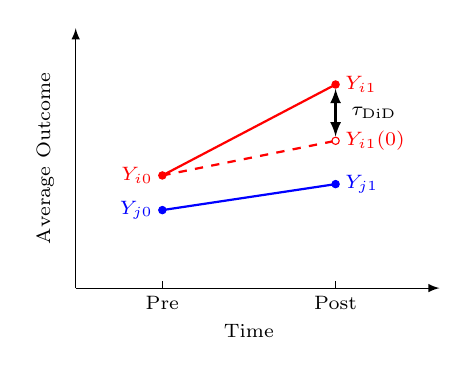
\begin{tikzpicture}[
        >=latex,
        scale=1.1,
        every node/.style={font=\scriptsize}
      ]

        % Axes ----------------------------------------------------
        \draw[->] (0,0) -- (4.2,0);    % x-axis
        \draw[->] (0,0) -- (0,3.0);    % y-axis

        % Axis labels
        \node[below]        at (2,-0.3)   {Time};
        \node[rotate=90]    at (-0.35,1.5) {Average Outcome};

        % Time points
        \coordinate (t0) at (1,0);
        \coordinate (t1) at (3,0);

        \draw (t0) -- ++(0,0.08) node[below=2pt] {Pre};
        \draw (t1) -- ++(0,0.08) node[below=2pt] {Post};

        % Control group (G = 0): observed outcomes ----------------
        \coordinate (C0) at (1,0.9);  % pre
        \coordinate (C1) at (3,1.2);  % post

        \draw[thick,blue] (C0) -- (C1);
        \filldraw[blue] (C0) circle (1.2pt);
        \filldraw[blue] (C1) circle (1.2pt);

        \node[blue,anchor=east]       at (C0) {$Y_{j0}$};
        \node[blue,anchor=west]       at (C1) {$Y_{j1}$};

        % Treated group (G = 1): observed outcomes ----------------
        \coordinate (T0) at (1,1.3);   % pre
        \coordinate (T1) at (3,2.35);  % post (treated)

        \draw[thick,red] (T0) -- (T1);
        \filldraw[red] (T0) circle (1.2pt);
        \filldraw[red] (T1) circle (1.2pt);

        \node[red,anchor=east]       at (T0) {$Y_{i0}$};
        \node[red,anchor=west]       at (T1) {$Y_{i1}$};

        % Counterfactual treated post (under parallel trends) -----
        \coordinate (T1cf) at (3,1.7); % same slope as control

        \draw[thick,red,dashed] (T0) -- (T1cf);
        \filldraw[red,fill=white] (T1cf) circle (1.2pt);

        \node[red,anchor=west] at (T1cf) {$Y_{i1}(0)$};

        % DiD effect as vertical distance -------------------------
        \draw[<->,thick]
          ($(T1cf)+(0,0.05)$) -- ($(T1)-(0,0.05)$)
          node[midway,right=2pt] {$\tau_{\text{DiD}}$};

      \end{tikzpicture}
      \vspace{0.15cm}

      \scriptsize Difference-in-differences in the $2 \times 2$ case.
    \end{column}
  \end{columns}
\end{frame}

\section{Synthetic Control}
%------------------------------------------------------------%

\begin{frame}{Setup}
  \begin{itemize}
    \item Alternative to parallel trends, focusing on a single treated unit.
    \item Panel with $N$ units over $T$ periods.
    \pause
    \item Single treated unit $N$ receiving treatment at time $T$:
    \begin{itemize}
      \item For $t = 1, \dots, T-1$: all units untreated,
      \[
        Y_{it} = Y_{it}(0), \quad i = 1,\dots,N.
      \]
      \item At $t = T$:
      \[
        Y_{iT} = Y_{iT}(0) \text{ for } i < N,
        \quad Y_{NT} = Y_{NT}(1).
      \]
    \end{itemize}
    \pause
    \item Causal estimand: the individual effect on unit $N$ at time $T$,
    \[
      \tau_N = Y_{NT}(1) - Y_{NT}(0) = Y_{NT} - \textcolor{magenta}{Y_{NT}(0)}.
    \]
    \item Problem: $\textcolor{magenta}{Y_{NT}(0)}$ is unobserved $\Rightarrow$ need to impute it.
  \end{itemize}
\end{frame}

%------------------------------------------------------------%

\begin{frame}{Convex Hull Assumption}
  \begin{itemize}
    \item We use the donor pool of control units $i = 1, \dots, N-1$ to approximate $Y_{Nt}(0)$.
    \pause
    \item \textbf{Assumption (Convex Hull).}
    There exist weights $(w_1,\dots,w_{N-1})$ with
      \[
        w_i \ge 0, \quad \sum_{i=1}^{N-1} w_i = 1
      \]
      such that for all $t = 1,\dots,T$,
      \[
        Y_{Nt}(0) = \sum_{i=1}^{N-1} w_i\, Y_{it}(0).
      \]
      \pause
    \item The treated unit’s untreated path is a \alert{time-invariant} weighted average of control paths.
  \end{itemize}
\end{frame}

\begin{frame}{Interpolation vs.\ Extrapolation}
  \begin{itemize}
    \item  Why do we insist on $ w_i \ge 0, \quad \sum_i w_i = 1?$
    \pause
    \item \textbf{Extrapolation:}
    \begin{itemize}
      \item The treated unit lies \emph{outside} the convex hull of controls.
      \item Unconstrained regression can predict far outside the range of the data.
    \end{itemize}
    \pause
    \item \textbf{Interpolation:}
    \begin{itemize}
      \item Project the treated unit into the convex hull of controls and predict \emph{within} a plausible region.
      \item This guards against wild predictions when we only care about a single treated unit.
    \end{itemize}
  \end{itemize}

  \vspace{0.3cm}

  \centering
  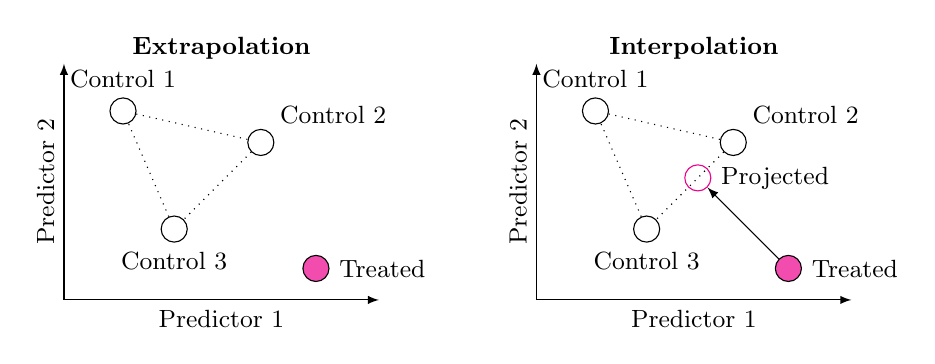
\begin{tikzpicture}[
    >=latex,
    scale=1,
    every node/.style={font=\small},
    control/.style={draw, circle, minimum size=5pt},
    treated/.style={draw, circle, fill=magenta!70, minimum size=5pt},
    cftreated/.style={draw=magenta, circle, minimum size=5pt}
  ]

    %------------------ Left panel: Extrapolation ------------------%
    \begin{scope}[xshift=0cm]
      % Axes
      \draw[->] (0,0) -- (4,0) node[midway, below] {Predictor 1};
      \draw[->] (0,0) -- (0,3) node[midway, above, rotate=90] {Predictor 2};

      % Title
      \node[font=\small\bfseries] at (2,3.2) {Extrapolation};

      % Controls
      \node[control,label=above:{Control 1}] (c1) at (0.75,2.4) {};
      \node[control,label=above right:{Control 2}] (c2) at (2.5,2.0) {};
      \node[control,label=below:{Control 3}] (c3) at (1.4,0.9) {};

      % Treated (outside convex hull)
      \node[treated,label=right:{Treated}] (tr) at (3.2,0.4) {};

      % Convex hull of controls
      \draw[dotted] (c1) -- (c2) -- (c3) -- (c1) -- cycle;
    \end{scope}

    %------------------ Right panel: Interpolation -----------------%
    \begin{scope}[xshift=6cm]
      % Axes
      \draw[->] (0,0) -- (4,0) node[midway, below] {Predictor 1};
      \draw[->] (0,0) -- (0,3) node[midway, above, rotate=90] {Predictor 2};

      % Title
      \node[font=\small\bfseries] at (2,3.2) {Interpolation};

      % Controls
      \node[control,label=above:{Control 1}] (c1) at (0.75,2.4) {};
      \node[control,label=above right:{Control 2}] (c2) at (2.5,2.0) {};
      \node[control,label=below:{Control 3}] (c3) at (1.4,0.9) {};

      % Treated
      \node[treated,label=right:{Treated}] (tr) at (3.2,0.4) {};
      % Projected / synthetic point inside convex hull
      \node[cftreated,label= right:{Projected}] (cf) at (2.05,1.55) {};

      % Arrow from treated to projection
      \draw[->] (tr) -- (cf);

      % Convex hull of controls
      \draw[dotted] (c1) -- (c2) -- (c3) -- (c1) -- cycle;
    \end{scope}

  \end{tikzpicture}
  \scriptsize
  Extrapolation (left) predicts using controls outside their convex hull; interpolation (right) projects into the convex hull of controls.
\end{frame}



\begin{frame}{Interpolation vs. Extrapolation}
  \begin{itemize}
    \item Example:
    \begin{itemize}
      \item All controls have unemployment between $5\%$ and $10\%$.
      \item Unconstrained regression could predict $20\%$.
      \item Synthetic control restricts predictions to $[5\%,10\%]$.
    \end{itemize}
    \pause
    \item As a prediction method for a single trajectory, avoiding extrapolation is crucial.
  \end{itemize}
\end{frame}

%------------------------------------------------------------%

\begin{frame}{Fitting the Synthetic Control}
  \begin{itemize}
    \item Choose $\hat w = (\hat w_1,\dots,\hat w_{N-1})$ to match the pre-treatment trajectory of unit $N$:
    \[
      \hat w = \arg\min_{w}
      \sum_{t=1}^{T-1}
      \left(
        Y_{Nt} - \sum_{i=1}^{N-1} w_i Y_{it}
      \right)^2
    \]
    subject to
    \[
      \sum_{i=1}^{N-1} w_i = 1, \quad w_i \ge 0 \ \forall i.
    \]
    \pause
    \item Counterfactual at $t = T$:
    \[
      \widehat Y_{NT}(0) = \sum_{i=1}^{N-1} \hat w_i Y_{iT}.
    \]
    \pause
    \item Synthetic control estimator:
    \[
      \hat\tau_N = Y_{NT} - \widehat Y_{NT}(0).
    \]
    \pause
    \item Works best with long, stable pre-treatment trajectories and a large donor pool.
  \end{itemize}
\end{frame}


\begin{frame}{Question}
\textbf{Important topics not discussed}:
\begin{itemize}
    \item RDD
    \item Double Robust Estimation
    \item Mediation
\end{itemize}
\vspace{1em}
 \centering
  {\Large \textbf{Any Questions?}}\\[1em]
  {\Large \textbf{Good luck!}}\\[1em]
  {\Large You’ve got this! Go show off those causal superpowers.}
\end{frame}







\end{document}
